\documentclass{book}%
\usepackage{amsfonts}
\usepackage{amsmath}%
\usepackage{graphicx}
\usepackage{epstopdf}
\usepackage{amssymb}%
\usepackage{hyperref}
\usepackage{textcomp}
\usepackage{listings}
\usepackage{units}
\usepackage{color}

\definecolor{dkgreen}{rgb}{0,0.6,0}
\definecolor{gray}{rgb}{0.5,0.5,0.5}
\definecolor{mauve}{rgb}{0.58,0,0.82}

\lstset{frame=tb,
  language=Python,
  aboveskip=3mm,
  belowskip=3mm,
  showstringspaces=false,
  columns=flexible,
  basicstyle={\small\ttfamily},
  numbers=none,
  numberstyle=\tiny\color{gray},
  keywordstyle=\color{blue},
  commentstyle=\color{dkgreen},
  stringstyle=\color{mauve},
  breaklines=true,
  breakatwhitespace=true,
  tabsize=3, upquote=true}

\lstMakeShortInline[columns=fixed]|




\setcounter{chapter}{1}

\begin{document}

\chapter[Statistical Representation of Data]{Communicating Results I: Statistical Representation of Data}

So far we have talked about repeating experiments, but we have been too
pressed for time to actually do that. We should take the time to see how to
report data from multiple results. Let's also tie the idea of multiple
results to our ideas of uncertainty.

To do this, I would like to go back to our dart board. Suppose I throw the
darts, trying for a bull's eye, and I get the following pattern:

\begin{center}
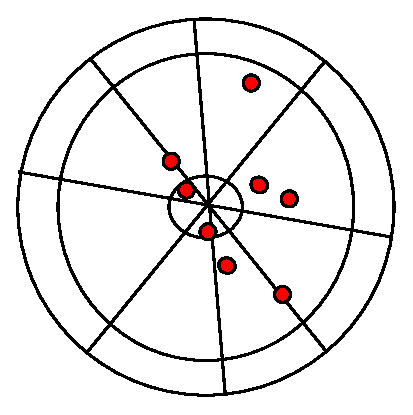
\includegraphics[scale=0.5]{Lab2_figs/bullseye_few.eps}
\end{center}

We now know that this is fairly accurate, but not very precise. We say that
there is a large uncertainty, but that we are aimed about the right
direction. We could get a better estimate of how accurate we are by
repeating the experiment many times:

\begin{center}
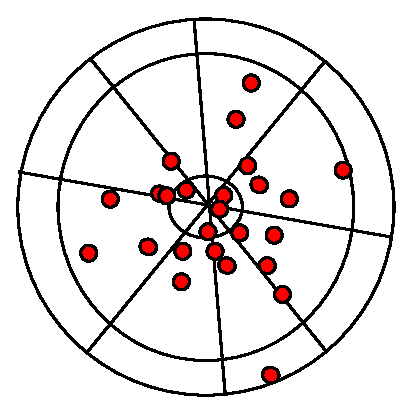
\includegraphics[scale=0.5]{Lab2_figs/bullseye_many.eps}
\end{center}

and finding an average location of the darts:

\begin{center}
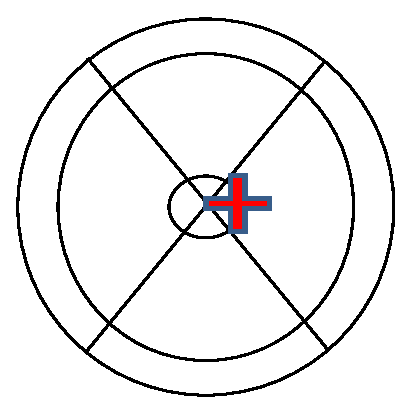
\includegraphics[scale=0.5]{Lab2_figs/bullseye_avg.eps}
\end{center}

This average seems to be just a little right of center. Now we know that we should point the darts a little
to the left. Many experiments are like this. We can repeat the experiment
many times. The uncertainty might be larger than we want, but if we average
over many trials of the experiment, we can find an average value that
represents the actual value of the quantity we are trying to find.

\section{Mean value as our best estimate value}

The mathematical process we use to find the mean is simple and you are
probably quite familiar with it. We simply add up all the values, and divide
the sum by the number of values.%
\begin{eqnarray*}
\bar{x} &=&\frac{x_{1}+x_{2}+x_{3}+\cdots x_{N}}{N} \\
&=&\frac{1}{N}\sum_{i=1}^{N}x_{i}
\end{eqnarray*}%
The last equation uses sigma notation. It is read as \textquotedblleft one
over $N$ times the sum of $x_{i}$ for $i=1$ to $N.$ It is a short-hand
notation for the line above. We will use this notation because it makes
writing our equations much easier. But that means it is very important that
we understand what it means. So let's imagine that we have many values for
the $x$-position for our darts.%
\[
\begin{array}{c}
x_{1}=1.00\pm 0.01\unit{cm} \\ 
x_{2}=0.50\pm 0.01\unit{cm} \\ 
x_{3}=-0.75\pm 0.01\unit{cm} \\ 
x_{4}=-2.25\pm 0.01\unit{cm} \\ 
x_{5}=3.00\pm 0.01\unit{cm} \\ 
x_{6}=-0.80\pm 0.01\unit{cm} \\ 
x_{7}=2.10\pm 0.01\unit{cm} \\ 
x_{8}=1.2\pm 0.01\unit{cm}%
\end{array}%
\]%
We have labeled each $x$ with a number. That is what the $x_{i}$ means. The
\textquotedblleft $i$\textquotedblright\ is an index. It stands for any
number from $1$ to $N.$ Our sigma notation says we add up all these
positions, and divide by $N=8$ since there are eight positions%
\begin{eqnarray*}
\bar{x} &=&\frac{\left( 1.00+0.50-0.75-2.25+3.00-0.80+2.10+1.2\right) \unit{%
cm}}{8} \\
&=&0.5\unit{cm}
\end{eqnarray*}%
which is a little bit to the right of our zero point.

\section{Standard deviation as an estimate of our uncertainty}

But what is our uncertainty? Each of our position measurements were good to $%
\pm 0.01\unit{cm}.$ But this can't be what governs our uncertainty. We can
see our points are spread out much more than $\pm 0.01\unit{cm}.$ Something
in the experiment (the bad dart thrower) is increasing the uncertainty. We
could use our algebraic method to find the uncertainty, but that would be
tedious and may not include the effects of the dart thrower. It would be
great to have a way to use the spread of the points, itself, to obtain a
numerical estimate of the uncertainty. The spread must include the effects
of the dart thrower.

From your study of statistics, you can guess what we will use to represent
uncertainty, but let's reason it out here. We could take how far each point
is from where we aimed as an indication of how imprecise our throw was. That
would be 
\[
\Delta x_{i}=\bar{x}-x_{i} 
\]%
for each throw. In this equation we are using the Greek $\Delta $ to show a
difference, and a bar over the $x$ to mean \textquotedblleft the average
value of the $x$-position.\textquotedblright\ Then $\Delta x_{i}$ is how far
off the $i^{th}$ trow from the mean. Sometimes we are off to the right, and
sometimes to the left. If we add up all the $\Delta x_{i}$ values and
average them, they will average to nearly zero most of the time. We can see
that zero is not a good estimate of our uncertainty! So the average
deviation won't work as a measure of uncertainty.

But we can play a trick. The quantity 
\[
\Delta x_{i}^{2}=\left( \bar{x}-x_{i}\right) ^{2} 
\]%
is always positive. If we averaged $\Delta x_{i}^{2},$ 
\[
\overline{\Delta x_{i}^{2}}=\frac{1}{N}\sum_{i=1}^{N}\Delta x_{i}^{2}=\frac{1%
}{N}\sum_{i=1}^{N}\left( \bar{x}-x_{i}\right) ^{2} 
\]%
nothing would cancel out. And we have solved our calcelation problem. But we
have created another problem by doing this, $\overline{\Delta x_{i}^{2}}$ is
like the square of our how far we are off. So let's take a square root%
\[
\sqrt{\overline{\Delta x_{i}^{2}}}=\sqrt{\frac{1}{N}\sum_{i=1}^{N}\Delta
x_{i}^{2}}=\sqrt{\frac{1}{N}\sum_{i=1}^{N}\left( \bar{x}-x_{i}\right) ^{2}} 
\]%
The quantity $\sqrt{\overline{\Delta x_{i}^{2}}},$ represents about how far
off we are on average, it does not tend to zero, and has the same units as $%
x_{i}$ so it can be an estimate of our uncertainty. It is about how far most
of the points are off from the mean. But $\sqrt{\overline{\Delta x_{i}^{2}}}$
is a little hard to write, so we usually give this quantity the symbol $%
\sigma $, which is a Greek letter $s$ and is pronounced \textquotedblleft
sigma.\textquotedblright\ We also give $\sigma $ a name. We call it the 
\emph{standard deviation} because it is about how much the average point
\textquotedblleft deviates\textquotedblright\ from the mean position. So for
our $x$-position we can write 
\[
\sigma _{x}=\sqrt{\sum_{i=1}^{N}\frac{\left( x_{i}-\bar{x}\right) ^{2}}{N}} 
\]%
But what does this math symbology mean? To find $\sigma _{x},$ we must first
find the average positions to find $\bar{x},$ then we take each $x$-position 
$\left( x_{i}\right) $ and we subtract the mean from it $\left( x_{i}-\bar{x}%
\right) .$ We square the result. We do this for each of our $x$-positions.
Then we have $\left( x_{1}-\bar{x}\right) ^{2},$ $\left( x_{2}-\bar{x}%
\right) ^{2},$ $\left( x_{3}-\bar{x}\right) ^{2},\cdots \left( x_{N}-\bar{x}%
\right) ^{2}.$ We add these up, and divide by $N$ to find the average $%
\sum_{i=1}^{N}\frac{\left( x_{i}-\bar{x}\right) ^{2}}{N}.$ Then we take the
square root.

In lab today, I\ will ask you to do this by hand once. That should be enough
to convince you that you never want to do it by hand again! Normally we will
use a computer to do this. I suggest you use one of our spreadsheet
programs, or python to do these calculations, and not your calculator.

\section{Histograms}

Suppose I\ plot the results of many, many dart throws. The way I want to
plot this is something you have seen from grading for many years. I want the
horizontal axis to show the $x$-position of the dart throws. I want the $y$%
-axis to show the number of darts that landed at a particular $x$-position.
This type of graph is called a histogram. You often see grades given like
this

\begin{center}
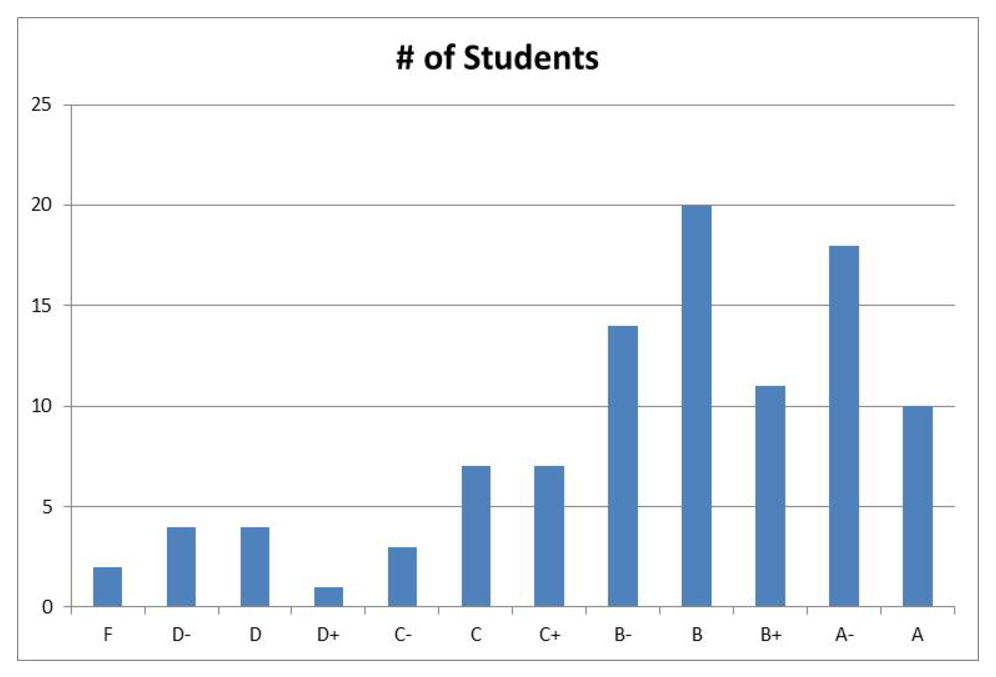
\includegraphics[scale=0.5]{Lab2_figs/hist_few.eps}
\end{center}

where we understand that the bars
indicate how many students got an $A$ (two in this case) and how many got an 
$A-$ (five in this case) etc.

If there are many students we can plot their scores and the shape of the
histogram begins to smooth out some

\begin{center}
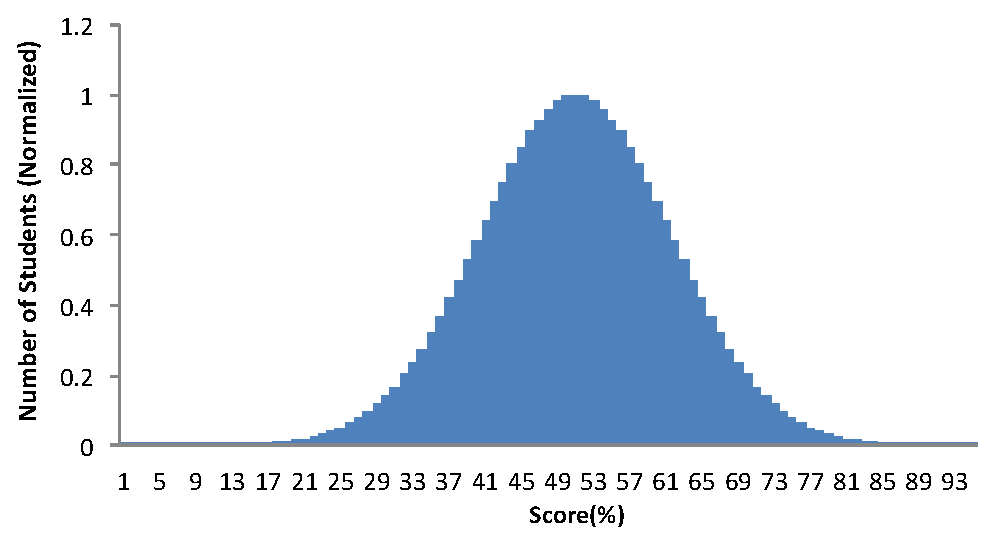
\includegraphics[scale=0.5]{Lab2_figs/hist_many.eps}
\end{center}

If we had infinitely many students, we would get a perfectly smooth curve.
You can see already that coloring in the bars in the graph is not useful any
more. So usually we just draw a point for the top of each bar. These points
form a curve.

\begin{center}
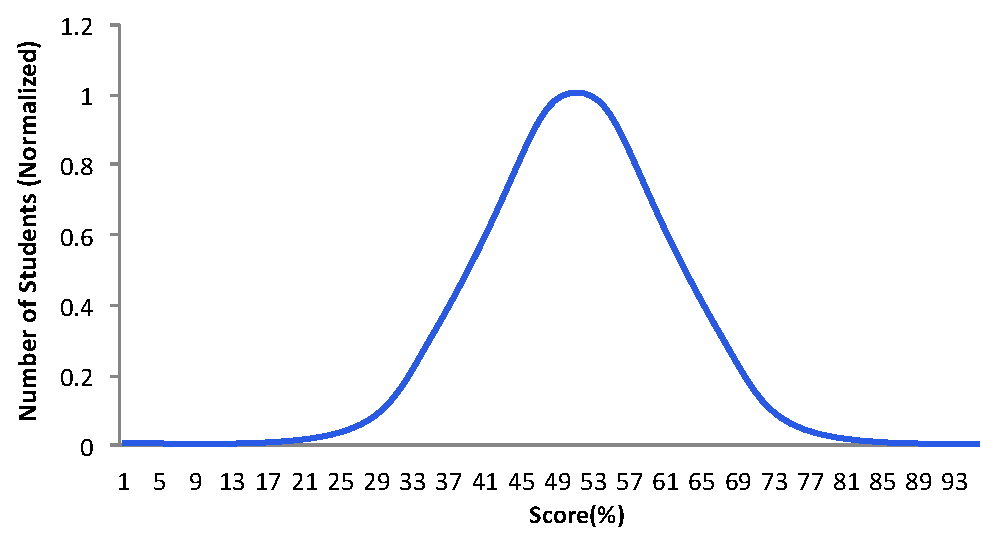
\includegraphics[scale=0.5]{Lab2_figs/hist_smooth.eps}
\end{center}

Unlike student scores, dart positions can be negative. So our dart
distribution should be centered on zero displacement. We will usually find
that $68\%$ of the darts will fall within $\pm \sigma $ of the mean. 

\begin{center}
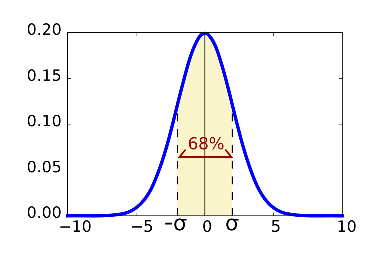
\includegraphics[scale=1.3]{Lab2_figs/normal_68.eps}
\end{center}

We can see that our $\sigma $ value is very like an uncertainty. But there
is a difference. We still have $32\%$ of our experiments outside of $\pm
\sigma ,$ and if we give the uncertainty, $\delta x,$ then all of the
measurements should be within $\pm \delta x.$ If you are building a space
shuttle and absolutely need to guarantee that your error on your calcuation
is within some limit, then you should use a true absolute uncertainty, $\pm
\delta x.$ But for most experiments, being that certain about our
uncertainty is not required, and we can use $\pm \sigma $ as a good
approximation to the uncertainty. We will often do this in this class. If
losing $32\%$ is not acceptable, but finding the true $\delta x$ is not
practical, it is often good enough to use $2\sigma $ or $3\sigma $ as the
estimate of our uncertainty. $95\%$ of the data will fall with $\pm 2\sigma
, $ and $99.7\%$ of the data will fall within $\pm 3\sigma .$ So these are
more conservative estimates than using a single standard deviation. But in
this class we will stick with just $\sigma .$

\section{Standard deviation of the mean}

Now you may wonder, does the mean value get better as we take more
measurements? That is, do we become more sure about where we are pointing if
we throw more darts and include these many darts' locations in our average?
I think you will see from our previous reasoning that this is the case. The
more trials of an experiment that we take, the closer our mean value is to
the \textquotedblleft truth\textquotedblright\ value we are measuring. Since
this is the case, shouldn't the uncertainty go down as we perform more
trials?

The answer is yes. We won't derive this in our class. But the estimate of
the uncertainty should be given by 
\[
\sigma _{\bar{x}}=\frac{\sigma _{x}}{\sqrt{N}} 
\]%
where $\sigma _{x}$ is our standard deviation in our $x$-position values and 
$N$ is the number of trials we took. The more trials that go into our
average, the lower our uncertainty estimate. The value $\sigma _{\bar{x}}$
is called the \emph{standard deviation of the mean}.

Notice that in some of our grade graphs, the most common score was not a $C.$
Here is an example: 

\begin{center}
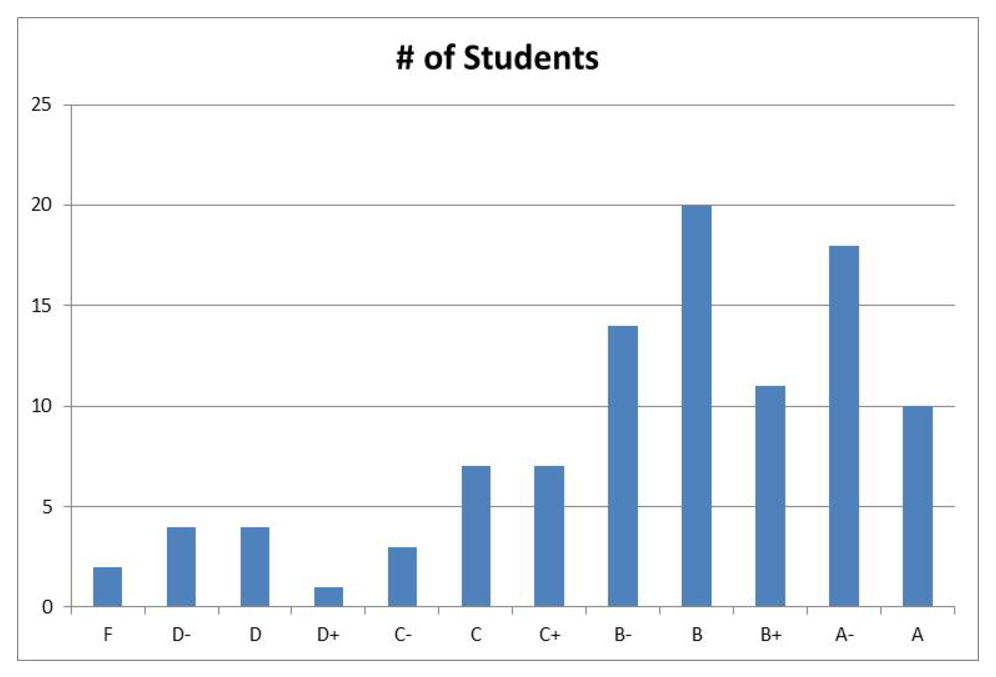
\includegraphics[scale=0.5]{Lab2_figs/hist_few.eps}
\end{center}

As students, this makes us all
happier, but for our error analysis this causes a problem. The error
analysis we have talked about so far assumes that our errors are distributed
in a very uniform way. If I go back to this graph

\begin{center}
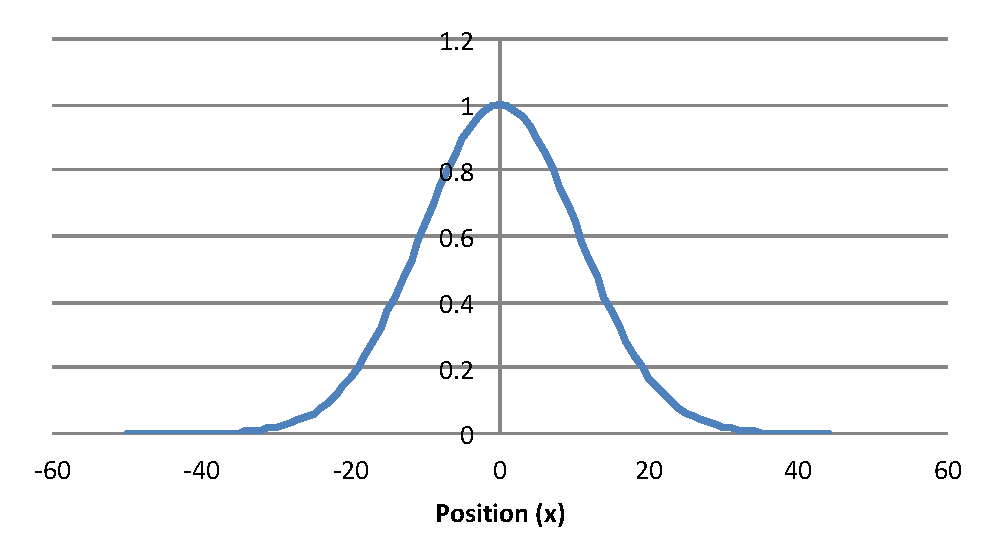
\includegraphics[scale=0.5]{Lab2_figs/hist_dart.eps}
\end{center}

we can see that there are as many
darts that landed to the left as there are to the right. This distribution
of errors is called the \emph{normal distribution}. Usually our errors in
our labs will be normally distributed. That makes all the math we talked
about work. But what if they are not, like our grade example? Well, that is
a great topic for PH336. So for now we will just assume a normal
distribution. But we can check to see how non-normal our data is. We can
find the \emph{mode} which is the value that occurs most frequently. For our
grade distribution above it would be a $B.$

We can also find the place where half of the trials landed on one side and
half on the other. This is called the \emph{median} point. We will calculate
both in our lab today. If we have a normal distribution, the average,
median, and the mode will all be the same. If this is not the case, then we
may worry a little about our error estimate--it may be too small.

\section{Graphical reporting of the mean (expected value) and standard
deviation (uncertainty)}

We now have a new view of measurement based on statistics. The mean value is
the value that we will say is our measurement. We call this the \emph{%
expected value}. The standard deviation is the representation of our
uncertainty. We can plot this in a way that communicates both at once. If we
take our eight data points that we started with earlier, we know the mean , $%
0.5\unit{cm},$ and we can find the standard deviation of the mean to be $0.6%
\unit{cm}.$ We plot this by making a dot or diamond or some larger point
indicator. Then we make a line through the point with little ends that show
the size of the uncertainty. The result looks like this.

\begin{center}
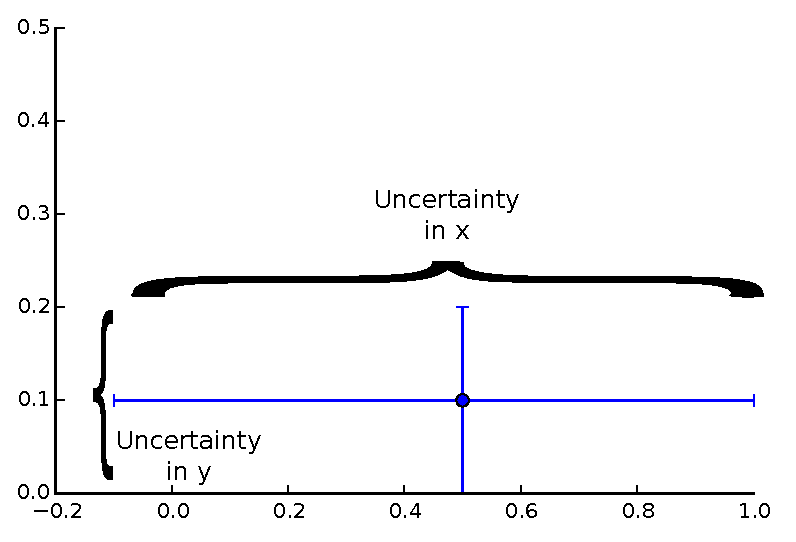
\includegraphics[scale=0.5]{Lab2_figs/error_bars.eps}
\end{center}

 Excel, and most plotting programs will allow you to
add error bars to your graphs.

Of course, we could have $y$
-direction error bars as well. These would be vertical, and there is no reason the $y$%
-error would be the same as the $x$-error. We may encounter such situations
in future labs.

\pagebreak

\section{Assignment}

Complete this lab in an organized fashion in your lab notebook. \emph{Part
of the grade will be based on neatness and organization!} There are several
histograms that need to be made during this lab. Make sure everyone in your
group gets a chance to build a histogram.

\subsection{Statistical Data I: How long does it take to walk?}

We will repeat one measurement, how long it takes to walk to a destination,
many times. Each person in our class will take the measurement once.

\begin{enumerate}
\item We'll start by determining a walking destination as a class. Our
destination is: \underline{\ \ \ \ \ \ \ \ \ \ \ \ \ \ \ \ \ \ \ \ }.

\item Each person in the class should get a digital timer and time their
walk to the destination and back. Walk at your normal walking speed. We will
stagger when you leave, to avoid walking in groups. While you are not
walking, you can begin working on part II.

\item When you return, record your walking time on the board to the nearest
second.

\item Record the times for all class members in a table
\item  \emph{by hand}
determine the mean walking time, the median walking time, and (if
appropriate) the modal walking time for the first 5 walkers. Determine the standard deviation of the
walking time of the first fve walkers\emph{by hand} (show all your work).

\item Using a computer: (see instructions below)
\begin{itemize}
\item 
\item confirm your mean walking time, median walking time, and (if appropriate) the modal walking time.
\item make a histogram of the walking times 
\end{itemize}
\end{enumerate}

\subsection{Making the Histogram in Python}
\subsubsection{Running your first Program}
Part of this class is learning to solve physics problems with a computer.  Today, you will be using the language python to find the median, and standard deviation of the walking data that we took.  Additionally, you will use it to make a histogram of the data.

When programming, it can be really helpful to make notes in your lab notebook about what each program does, things you learned about different functions, etc.  At the bare minimum you should include you final program, any graphs it makes, as well as where you saved it, and what name you saved it under.  That will make it easier to find in the future.

To begin writing your program, open up your favorite plain text editor.  I like notepad++ for windows or text wrangler on mac. Or, if you downloaded python from Enthought or Anaconda you can use Canopy (Enthought) or Spyder (Anaconda).   Enter the walking data like so: (Be sure to use the class data, not this sample data.)

\begin{lstlisting}[language=Python]
#Our walking data
data = [34, 38, 33, 38, 38, 36, 35, 47,36, 32, 40, 40, 
       45, 36, 43, 38, 48, 40, 40, 38, 43, 40, 39, 36, 46, 
       34, 37, 33, 32, 34 ]
print(data)

\end{lstlisting}
The first line is called a comment.  The |\#| tells the python interpreter (the thing that runs python) to ignore that line.  You should use comments to describe what your are doing in your program, that way you remember what it was later, or if anyone else has to read it they'll know what you did.  There will not be any more example comments in this tutorial.  You will have to come up with your own.

Let's look at the next set of lines:
\begin{lstlisting}[language=Python]
data = [34, 38, 33, 38, 38, 36, 35, 47,36, 32, 40, 40, 
       45, 36, 43, 38, 48, 40, 40, 38, 43, 40, 39, 36, 46, 
       34, 37, 33, 32, 34 ]
\end{lstlisting}
They load our walking data into what is called a list.  It's a way to save our data under a different name for easier access.
The |print(data)| command tells the computer to print out what we've saved in data.  

Save your file with the extension |.py|. (Example: |myFile.py|)  That tells your computer that it is a python script.

If you are using Canopy or Spyder, you can run your script by clicking play or hitting f5.  If you aren't using one of those, open up your command line on Windows or the terminal on Linux or Mac.  Navigate the where you saved your file (ask the instructor for help if you need it) and type in the command:
\begin{lstlisting}
python 'myFile.py'
\end{lstlisting}
but insert your file name. That tells your computer to run the python script.  You should see your data printed out on the screen.

\subsubsection{Finding the Mean, Median, and Standard deviation}

First, remove the |print(data)| line from your program. We don't need to have the computer spit that out again and again.  

Add these lines to your script:
\begin{lstlisting}[language=python]
import numpy as np
dataMean=np.sum(data)/len(data)
print('Mean:  {0:.2f}'.format(dataMean))
\end{lstlisting}

The first line loads a module called numpy.  Python keeps a lot of functions in separate modules.  Loading one is sort of like grabbing a book with the right set of instructions in it.  Now, all of the numpy functions are stored in the letters |np|.

The next line creates a variable called |dataMean|. The numpy sum command adds up all of the values in |data|, and |len(data)| gives you how many items are in the |data| list. (|len| is short for length).  

The third line prints |dataMean|.  Save your program again and run it to see what happens.  Try changing the 2 in the print command line to a three, save it, run it again, and see what has changed.

Numpy has a function that will calculate the mean for you.  Here's our script from above with one addition: |dataMeanNp| gives the mean of the data as calculated by numpy.
\begin{lstlisting}[language=python]
import numpy as np
dataMean=np.sum(data)/len(data)
print('Mean:  {0:.2f}'.format(dataMean))
dataMeanNp=np.mean(data)
print('Numpy Mean:  {0:.2f}'.format(dataMeanNp))
\end{lstlisting}


Your assignment for this part is to {\em add} these parts to your program:
\begin{enumerate}
\item a part where the program calculates and prints the standard deviation using the formula in the reading.
\item a part that uses numpy to find the median and standard deviation of our walking data.  The numpy function that finds the median is |median| and the numpy function that finds the standard deviation is |std|.
\end{enumerate}
Once you find the median and standard deviation, tell your script to print the median with no decimal places and to print the standard deviation to three decimal places. 

You should also include {\em comments} in your program.  Comments are notes for people to read, but that the computer will ignore.  You can start a comment with the |\#| character.  Part of keeping a good lab notebook is printing out copies of your programs, complete with comments. Here's the example program, all in one place, with good comments added:
\begin{lstlisting}[language=python]
#Load the class walking times into the variable "data"
data = [34, 38, 33, 38, 38, 36, 35, 47,36, 32, 40, 40, 
       45, 36, 43, 38, 48, 40, 40, 38, 43, 40, 39, 36, 46, 
       34, 37, 33, 32, 34 ]
       
#Importing the numpy library for easy calculations
import numpy as np

#Calculate the mean of data using the mean formula 
dataMean=np.sum(data)/len(data)
#Print the mean as a float with two decimal places
print('Mean:  {0:.2f}'.format(dataMean))

#Calculate the mean of the data using numpy's mean function
#If I did dataMean correctly, dataMeanNp should give the same result
dataMeanNp=np.mean(data)
#Print the mean calculated from numpy's function.  
print('Numpy Mean:  {0:.2f}'.format(dataMeanNp))
\end{lstlisting}

\subsubsection{Making a histogram}

Adding the following code to your script to make the histogram:

\begin{lstlisting}[language=python]
import matplotlib.pyplot as plt
plt.hist(data, 20, normed=0, facecolor='green', alpha=0.75)

plt.xlabel('My x axis Label')
plt.ylabel('My y axis label')
plt.title('My Title')
plt.savefig('myPlot.pdf')
\end{lstlisting}

This script will make a histogram with 20 bins and save it to the file |myPlot.pdf|.  In your program you should:
\begin{itemize}
\item Change the number of bins to something more appropriate for your data. If your fullest bin only has one or two items in it, you have way too man bins.  If everything fits into three or four bins, you have too few.  
\item Fix the plot title and axis labels to match what {\em you} are plotting. 
\item Add appropriate comments. If you have enough comments, it can be very helpful to refer back to this program in future weeks.  If you don't have enough, you will forget what this program does, and it won't be helpful to you.
\end{itemize}

Print out your completed program and histogram and add them to your lab notebook.
\end{document}
